\documentclass{beamer}

\usepackage[utf8]{inputenc}
\usepackage{listings}
\usepackage{ulem}
\usepackage{hyperref}
\usepackage{amsmath}

\hypersetup{
    colorlinks=true,
    linkcolor=white,
    filecolor=magenta,      
    urlcolor=cyan,
}
 
\usetheme{Dresden}

\title[COMPSCI 235 Lab 2 (2020)]
{Git / HTML / CSS}
  
\author{Nisarag Bhatt / Bill Bao}
 

\date[Auguest 2020]{COMPSCI235 Lab 2}

\begin{document}
\setbeamertemplate{caption}{\raggedright\insertcaption\par}

\frame{\titlepage}


\section{Learning Outcomes}
\begin{frame}
  \frametitle{Learning Outcomes}
  \begin{itemize}
  	\item Make a Github Account
    \item Install Git on your computer
    \item Create a repository with Github and Git
    \item Using Git to clone/add/commit/push/fork
    \item Edit HTML and CSS Files
    \end{itemize}
\end{frame}



\section{Github and Git}

\begin{frame}
  \frametitle{Why use Git?}
  
  Have you ever had assignments named:
  
  \begin{itemize}
  	\item \texttt{assignment.py}
  	\item \texttt{assignment-final.py}
  	\item \texttt{assignment-actual-final.py}
  	\item \texttt{assignment-submission.py}
  	\item \texttt{assignment-final-final-submission.py}
  \end{itemize}
  
  \pause 
  
  Well, Git tracks the changes you make to files, so you have a record of what has been done, and you can revert to specific versions should you ever need to. 
\end{frame}

\begin{frame}
  \frametitle{Usage of Git throughout the course}
  
  \begin{itemize}
  	\item You will be using Git to track your files through some of the assignments
  	\item You will also be submitting few assignments through Github so it is vital that you understand it 
  \end{itemize}
  
  
  
\end{frame}

\begin{frame}
  \frametitle{Git vs Github}
  	\begin{figure}
		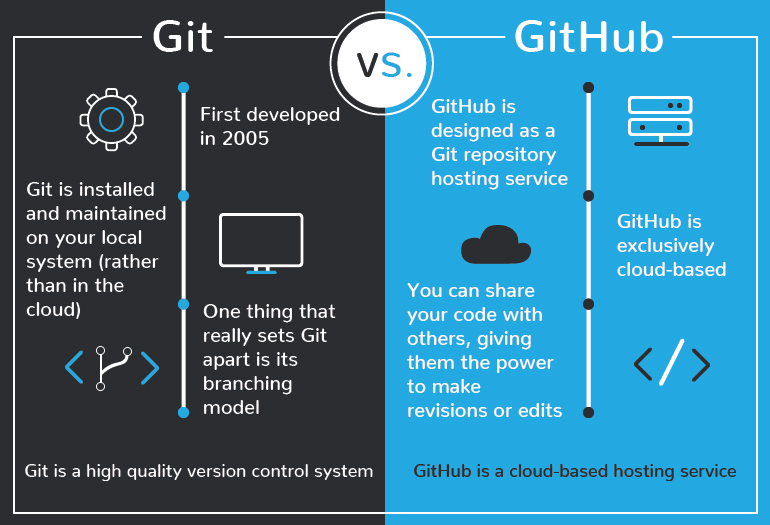
\includegraphics[scale=0.3]{./git-vs-github}
		\caption{Source of Image \href{https://blog.devmountain.com/git-vs-github-whats-the-difference/}{here}}
	\end{figure}
\end{frame}


\begin{frame}
  \frametitle{Installing Git}
  \begin{itemize}
    	\item Windows Users	
    	\begin{itemize}
  			\item Download from \href{https://git-scm.com/download/win}{https://git-scm.com/download/win}
  		\end{itemize}
  		\item Mac Users	
    	\begin{itemize}
  			\item Check Git is installed by going to Terminal and running the command: \texttt{git --version}
  			\item If it doesn't show a version then you need to install Git, To do this download \href{Homebrew}{https://brew.sh/} which is a package manager by running the specified command on terminal
  			\item Once Homebrew is installed run the command: \texttt{brew install git}
  			\item Run \texttt{git --version} once again to ensure Git has been installed
  		\end{itemize}
  \end{itemize}
\end{frame}

\begin{frame}
\frametitle{Configuring Git}
	Run these commands on the Terminal: 
	\linebreak

  \texttt{git config --global user.email your email@gmail.com} \\ 
  \texttt{git config --global user.name your-name}\\ 
  \texttt{git config --global credential.helper store} \\ \_\\If you want you can use SSH keys for a more secure way of saving your credentials but for this tutorial this should be sufficient.
\end{frame}

\begin{frame}
	\frametitle{Creating a new repository}
	\begin{itemize}
		\item Go to your profile and click on the "Repositories" tab 
		\item Create new repository named: \{your-upi\}-235-lab2
		\item Give it an optional description
		\item Make sure the repository is public
		\item Make sure you have ticked "Initialize this repository with a README"
		\item Click on "Create Repository"
	\end{itemize}
\end{frame}


\begin{frame}
  \frametitle{Clone}
  \begin{itemize}
  	\item Go to your repository and find its url and copy that
  	\begin{figure}
		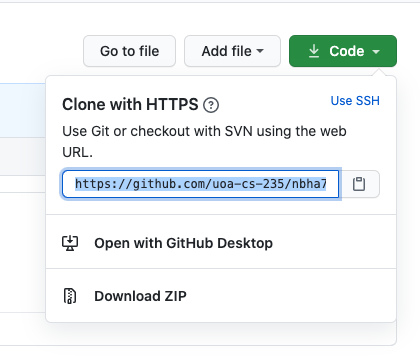
\includegraphics[scale=0.3]{./git-url}
	\end{figure}
	\item Go to your terminal and run: \texttt{git clone <the url>} in a directory of your choice
 \end{itemize}
\end{frame}

\begin{frame}
  \frametitle{Editing and Pushing to Github}
  \begin{itemize}
  	\item In one of these steps you may be asked for your Github Username and Password.
  	\item Open up the README.md file and add some text introducing yourself
  	\item Once this is done go back to the terminal
  	\item Run \texttt{git add README.md}
  	\item Run \texttt{git commit -m "Adding introduction to readme"}
  	\item Run \texttt{git push} to actually push this change to your Github
  	\item Link this repository on your lab report so we can make sure that you have completed this part of the excercise.
 \end{itemize}
\end{frame}


\section{HTML + CSS}

\begin{frame}
  \frametitle{Forking a Repository}
  \begin{itemize}
  	\item When you fork a repository, you are copying that repository into your own personal account
  	\item Daniel has made a repository to practice with: \href{https://github.com/senddanemail/coffeebeanroast}{github.com/senddanemail/coffeebeanroast} so fork that to your account with the button on the top right corner 
  	\begin{figure}
  	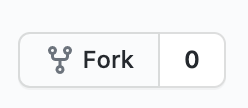
\includegraphics[scale=0.5]{./fork}
	\end{figure}
  	\item Go to your account and under repositories you will see that there is a copy of the repo you just forked
  	\item You now clone this into your account by following the same steps as above
 \end{itemize}
\end{frame}

\begin{frame}
  \frametitle{Playing around with HTML + CSS}
  \begin{itemize}
  	\item Open the project up in PyCharm
  	\item Start running the project in your browser, make sure you can see the project running. Try understand how the HTML and CSS make up the page you see.
  	\item Go to \href{https://bit.ly/31EWDEs}{this} link to validate the HTML. When you paste the HTML you should see a few errors 
  	\begin{figure}
  	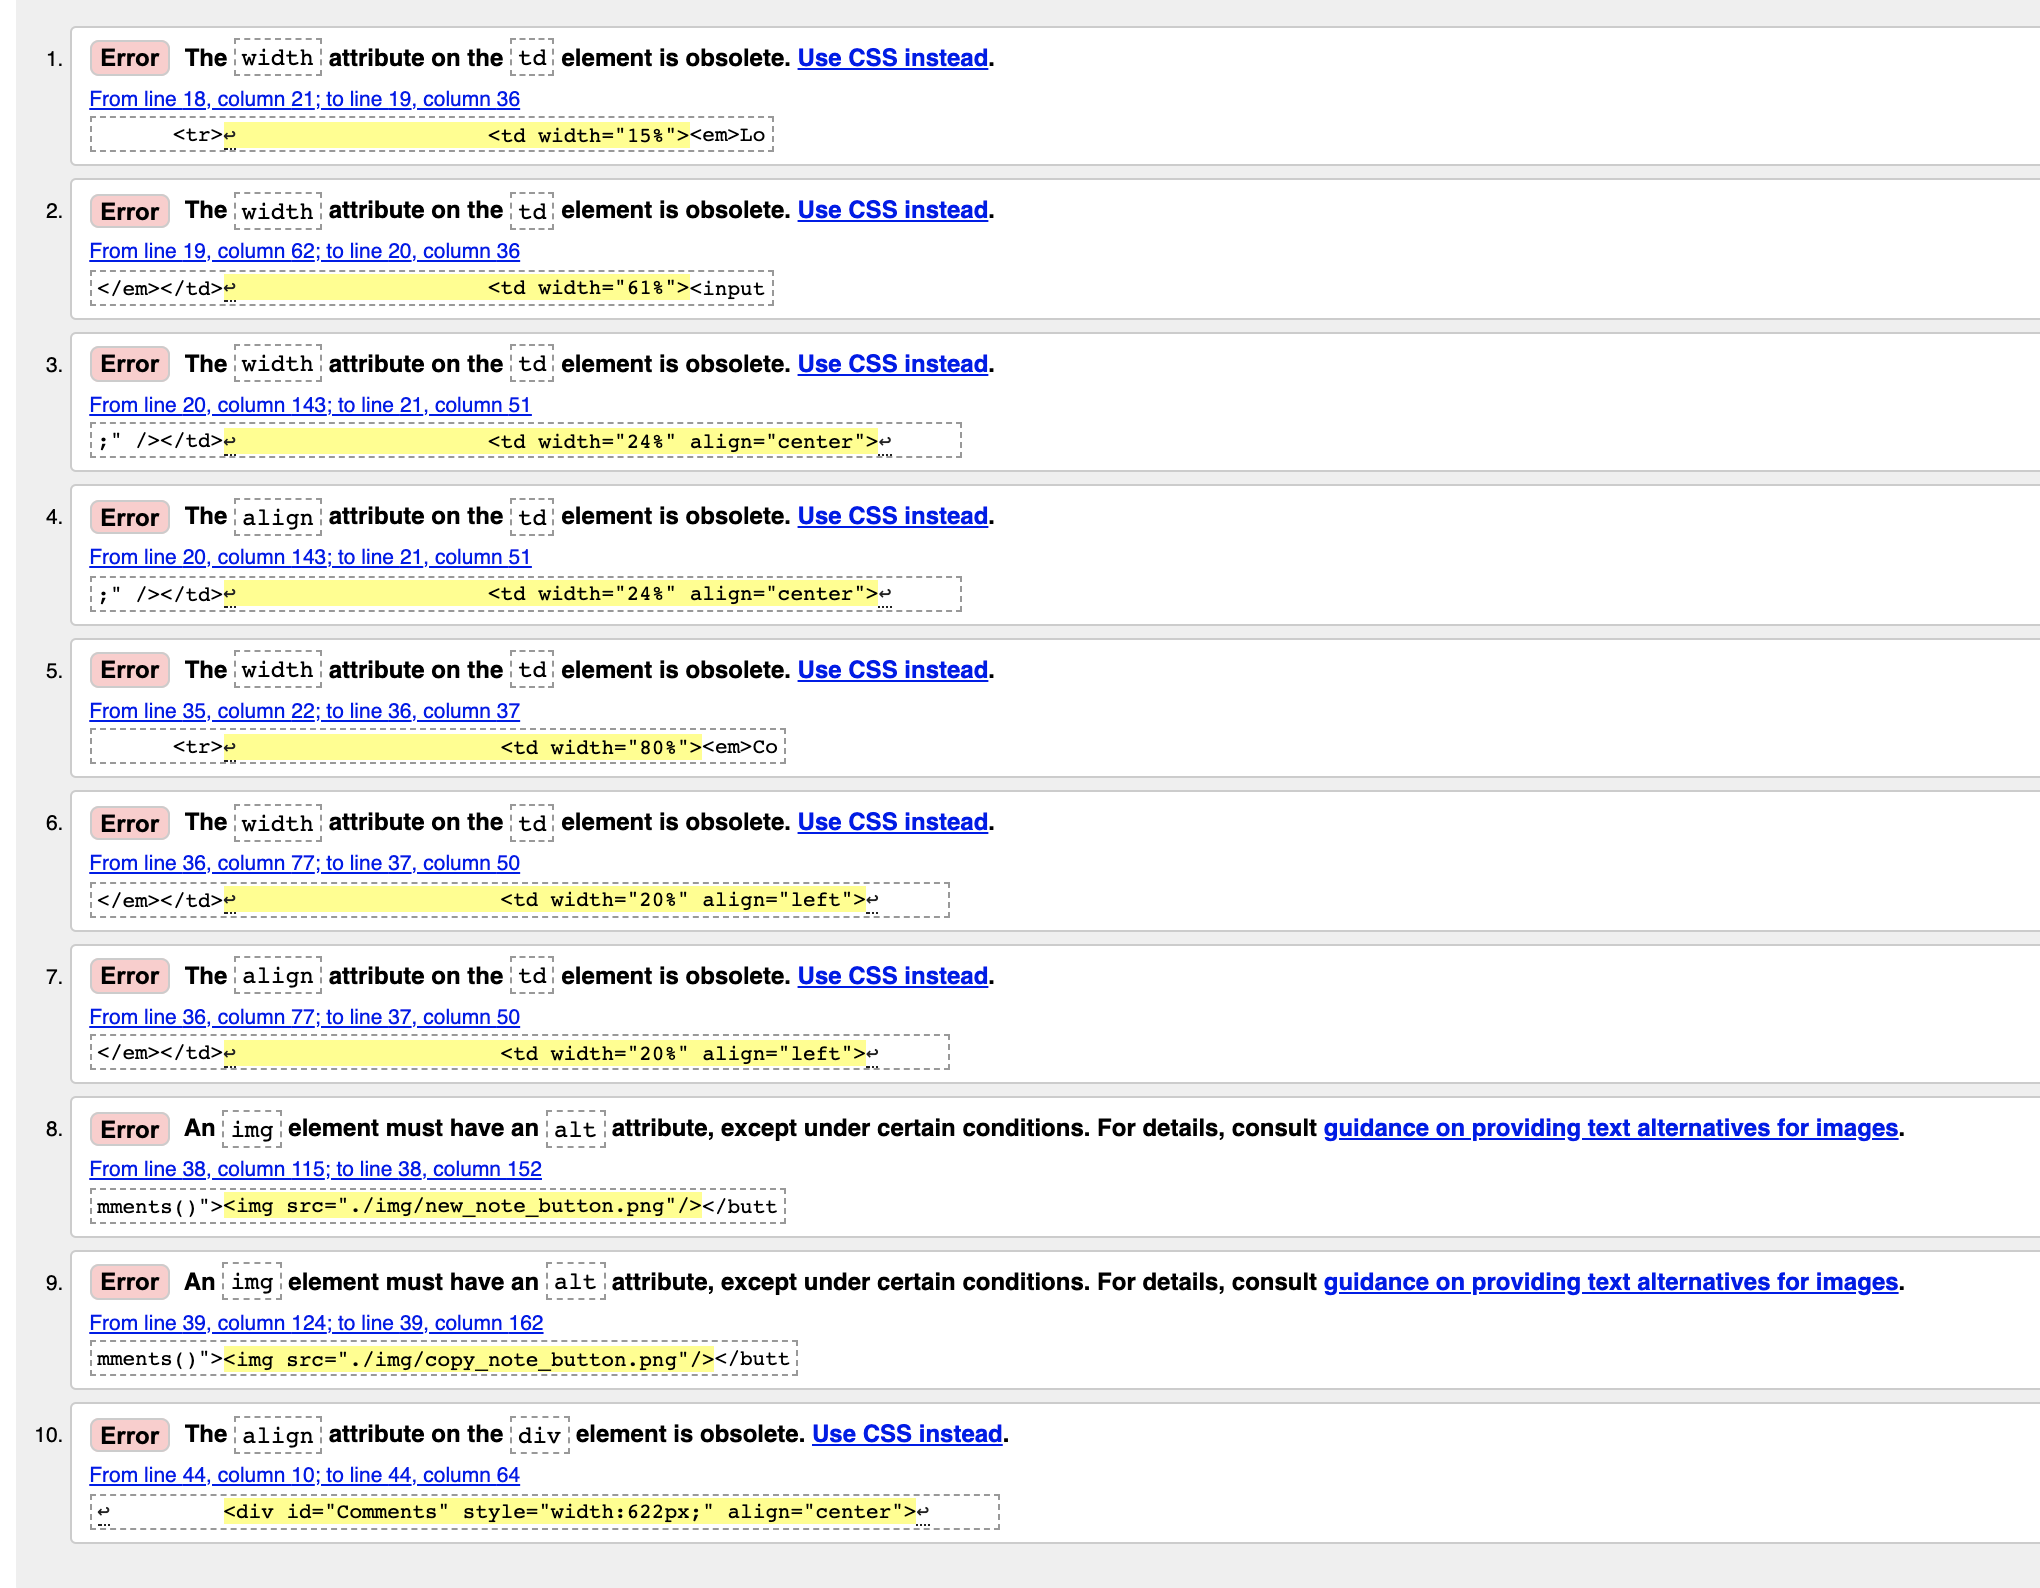
\includegraphics[scale=0.1]{./errors}
	\end{figure}
 \end{itemize}
\end{frame}


\begin{frame}
  \frametitle{Fixing errors}
  \begin{itemize}
  	\item Go through the errors and try fix them one by one
  	\item They provide some good hints such as making css id / classes instead of hard coding the styles
  	\item The alt attribute provides alternative information for an image if a user for some reason cannot view it (because of slow connection, an error in the src attribute, or if the user uses a screen reader).
  	\item The images \textbf{do not} have alt attributes so it is good to add a meaningful one
  	\item At the end you should have no errors. Once this is done, push your changes to your Github like before and share the link with us in your report, we will be checking your code.
 \end{itemize}
\end{frame}

\begin{frame}
  \frametitle{Useful Resources}
  \begin{itemize}
  	\item \href{https://www.youtube.com/watch?v=SWYqp7iY_Tc}{Git and Github Crash Course}
  	\item \href{https://www.youtube.com/watch?v=USjZcfj8yxE}{Learn Git in 15 minutes!}
  	\item \href{https://www.youtube.com/watch?v=wXUhTZpF_HQ}{Introduction to Classes and IDs in HTML}
 \end{itemize}
\end{frame}




\end{document}
